\documentclass[tikz,border=8pt]{standalone}

\usepackage[T1]{fontenc}
\usepackage[utf8]{inputenc}
\usepackage{lmodern}
\usetikzlibrary{arrows.meta,positioning}

\definecolor{distBlue}{RGB}{30,90,200}
\definecolor{varRed}{RGB}{176,20,30}
\definecolor{cvarFill}{RGB}{252,190,190}
\definecolor{pruneGray}{RGB}{150,150,150}

\begin{document}
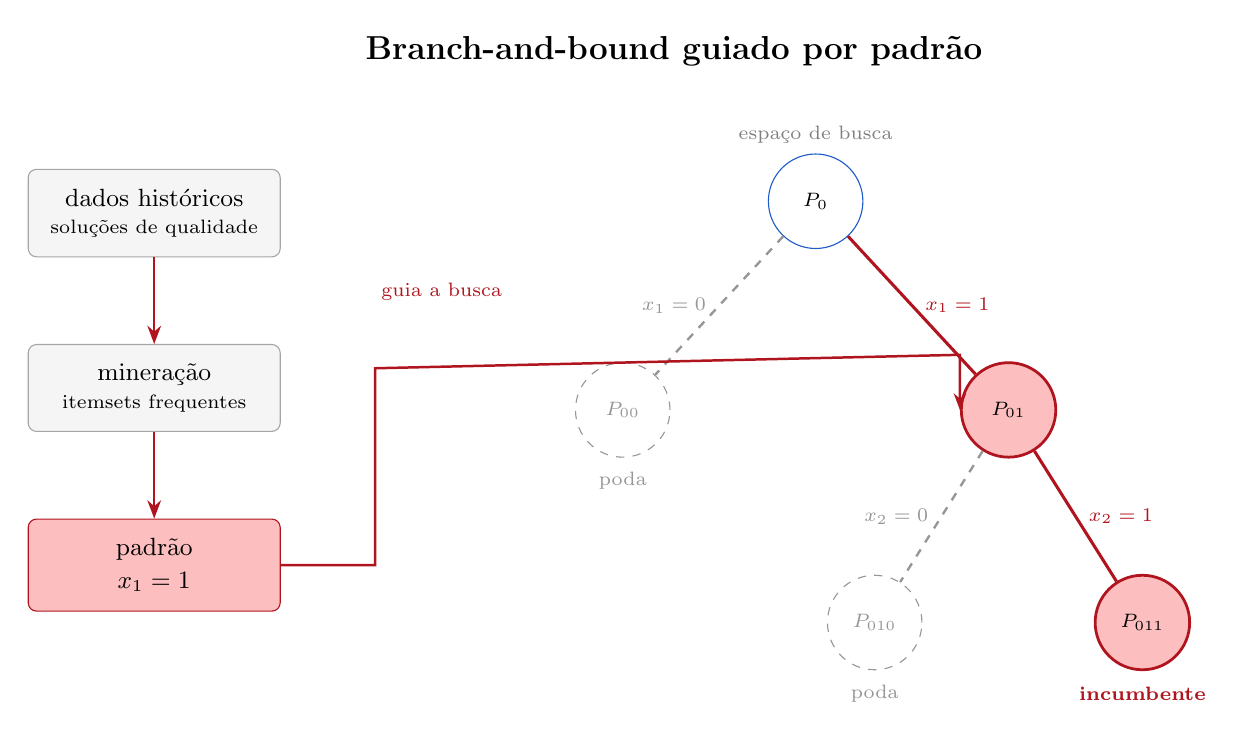
\begin{tikzpicture}[
  font=\small,
  >=Stealth,
  box/.style={
    draw=black!35,
    rounded corners=3pt,
    align=center,
    inner sep=7pt,
    minimum width=3.2cm,
  },
  nd/.style={
    draw=distBlue,
    fill=white,
    circle,
    inner sep=1pt,
    minimum size=12mm,
    font=\scriptsize,
    align=center,
  },
  ndhot/.style={
    nd,
    draw=varRed,
    fill=cvarFill,
    line width=1pt,
  },
  ndcut/.style={
    nd,
    draw=pruneGray,
    dashed,
    text=pruneGray,
  },
]

  \node[font=\bfseries\large] at (6.8,8.6)
    {Branch-and-bound guiado por padr\~ao};

  \node[box, fill=black!4] (dados) at (0.2,6.55)
    {dados hist\'oricos\\[-1pt]{\scriptsize solu\c{c}\~oes de qualidade}};
  \node[box, fill=black!4, below=11mm of dados] (mine)
    {minera\c{c}\~ao\\[-1pt]{\scriptsize itemsets frequentes}};
  \node[box, fill=cvarFill, draw=varRed, below=11mm of mine] (pad)
    {padr\~ao\\[1pt]{$x_1=1$}};

  \draw[->, thick, varRed] (dados) -- (mine);
  \draw[->, thick, varRed] (mine) -- (pad);

  \node[nd] (p0) at (8.6,6.7) {$P_0$};
  \node[ndcut] (p00) at (6.15,4.05) {$P_{00}$};
  \node[ndhot] (p01) at (11.05,4.05) {$P_{01}$};
  \node[ndcut] (p010) at (9.35,1.35) {$P_{010}$};
  \node[ndhot] (p011) at (12.75,1.35) {$P_{011}$};

  \draw[pruneGray, dashed, line width=0.85pt] (p0) -- (p00)
    node[midway, left, font=\scriptsize, pruneGray, xshift=-1pt] {$x_1=0$};
  \draw[varRed, line width=1.1pt] (p0) -- (p01)
    node[midway, right, font=\scriptsize, varRed, xshift=1pt] {$x_1=1$};
  \draw[pruneGray, dashed, line width=0.85pt] (p01) -- (p010)
    node[midway, left, font=\scriptsize, pruneGray, xshift=-1pt] {$x_2=0$};
  \draw[varRed, line width=1.1pt] (p01) -- (p011)
    node[midway, right, font=\scriptsize, varRed, xshift=1pt] {$x_2=1$};

  \node[font=\scriptsize, pruneGray] at (6.15,3.15) {poda};
  \node[font=\scriptsize, pruneGray] at (9.35,0.45) {poda};
  \node[font=\scriptsize\bfseries, varRed] at (12.75,0.45) {incumbente};

  \draw[varRed, -{Stealth[length=6pt]}, line width=0.9pt]
    (pad.east) -- ++(1.2,0) -- ++(0,2.5)
    -- ([yshift=7mm] p01.west) -- (p01.west);

  \node[font=\scriptsize, varRed] at (3.85,5.55) {guia a busca};

  \node[font=\scriptsize, text=black!50] at (8.6,7.55)
    {espa\c{c}o de busca};

\end{tikzpicture}
\end{document}
